% slides.tex
\documentclass[20pt]{beamer}
\usepackage{listings}
\usepackage[utf8]{inputenc}
\usepackage{color}
\usepackage{graphicx}

\usetheme{default}
\usecolortheme{dove}
\useoutertheme{default}

% Slightly smaller title
\setbeamerfont{frametitle}{size=\large}
\setbeamerfont{verb}{size=\small}

% lst settings
\lstset{
    language=Haskell,
    basicstyle=\small,
    gobble=4
}

\newcommand{\vspaced}{
    \vspace{5mm}
}

\begin{document}

\title{The Haskell WebSockets library}
\subtitle{Dutch HUG Day}
\author{Jasper Van der Jeugt}
\date{April 20, 2012}

\begin{frame}[plain]
    \titlepage
\end{frame}

% Introduction
% ------------

\begin{frame}{Hello!}
    My name is Jasper \\
    Student at UGent \\
    I write Haskell \\
    GhentFPG \\
    \texttt{@jaspervdj} \\
    \texttt{jaspervdj.be}
    \begin{picture}(0.0, 0.0)
    \put(40.0, -15.0){
        
\includegraphics[width=0.5\textwidth]{../2011-functionalpx-blaze-html/images/hat.pdf}}
    \end{picture}
\end{frame}

% About WebSockets
% ----------------

\begin{frame}{Overview}
    \textbf{About WebSockets} \\
    Protocol versions: typeclass fun \\
    Example: a webchat \\
\end{frame}

\begin{frame}{WebSockets}
    \textbf{WebSocket} is a web technology providing bi-directional, full-duplex
    communication channels, usually between a browser and an HTTP server.
\end{frame}

\begin{frame}[fragile]{WebSockets}
    Starts as an HTTP request, usually over port 80
    \vspaced
    \begin{lstlisting}
    GET /chat HTTP/1.1
    Host: server.example.com
    Upgrade: websocket
    Connection: Upgrade
    ...
    \end{lstlisting}
\end{frame}

\begin{frame}[fragile]{WebSockets}
    Server upgrades the connection
    \vspaced
    \begin{lstlisting}
    HTTP/1.1 101 Switching Protocols
    Upgrade: websocket
    Connection: Upgrade
    ...
    \end{lstlisting}
\end{frame}

\begin{frame}{WebSockets}
    Possible uses: \\
    \vspaced
    Chat services \\
    Multiplayer games \\
    Real-time notifications \\
    ...
\end{frame}

\begin{frame}[fragile]{WebSockets}
    \begin{lstlisting}
    var ws = new WebSocket(uri);
    ws.onmessage = function(event) {
        alert(event.data);
    };
    ws.onmessage = function() {
        ws.send('Hello, server.');
    };
    \end{lstlisting}
\end{frame}

\begin{frame}{About WebSockets}
    Supported browsers:
    \begin{center}
    
\includegraphics[width=0.9\textwidth]{images/browsers.png}
    \end{center}
    IE10 will also support the protocol
\end{frame}

% Protocol versions: typeclass fun
% --------------------------------

\begin{frame}{Overview}
    About WebSockets \\
    \textbf{Protocol versions: typeclass fun} \\
    Example: a webchat \\
\end{frame}

\begin{frame}{Protocol versions: typeclass fun}
    Two main versions in use: \\
    hybi-00 and hybi-10 \\
    \vspaced
    \small{(other versions are similar)} \\
\end{frame}

\begin{frame}{About WebSockets}
    Important detail: \\
    \vspaced
    Protocol allows for version negotiation between client and server
\end{frame}

\begin{frame}{Protocol versions: typeclass fun}
    Features:
    \begin{center}
    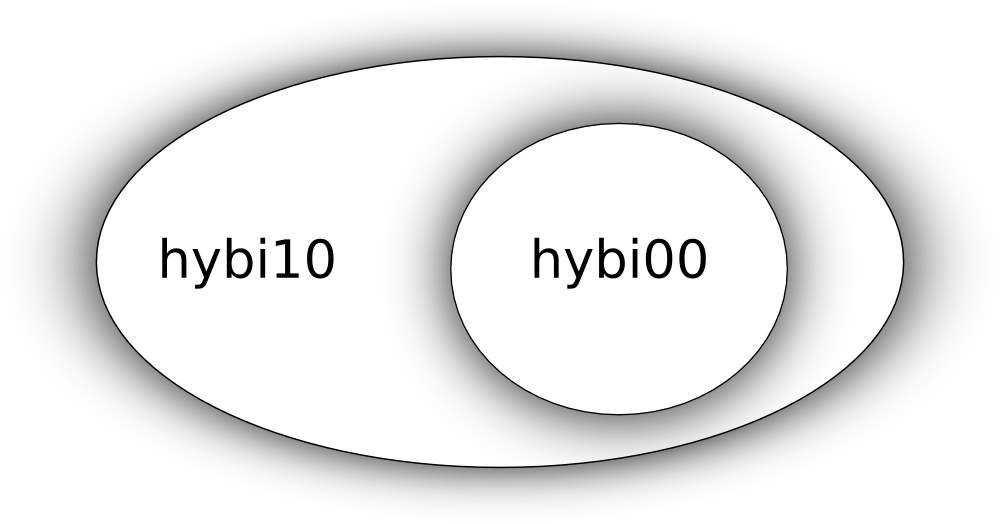
\includegraphics[width=\textwidth]{images/features.png}
    \end{center}
\end{frame}

\begin{frame}{Protocol versions: typeclass fun}
    Implementation:
    \begin{center}
    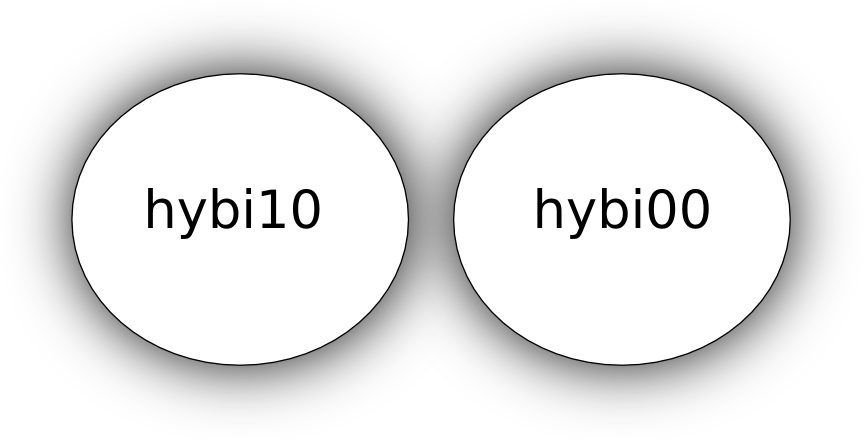
\includegraphics[width=\textwidth]{images/implementation.png}
    \end{center}
\end{frame}

\begin{frame}{Protocol versions: typeclass fun}
    Code on the following slides is simplified for conciceness and clarity...
\end{frame}

\begin{frame}[fragile]{Protocol versions: typeclass fun}
    \begin{lstlisting}
    sendTextData
      :: TextProtocol p
      => Text
      -> WebSockets p ()
    \end{lstlisting}
\end{frame}

\begin{frame}[fragile]{Protocol versions: typeclass fun}
    \begin{lstlisting}
    sendBinaryData
      :: BinaryProtocol p
      => ByteString
      -> WebSockets p ()
    \end{lstlisting}
\end{frame}

\begin{frame}[fragile]{Protocol versions: typeclass fun}
    \begin{lstlisting}
    -- Compatible with hybi-00
    -- and hybi-10
    app :: TextProtocol p
        => WebSockets p ()

    main :: IO ()
    main = serve
      -- Use hybi-00 or above
      (app :: WebSockets Hybi00 ())
    \end{lstlisting}
\end{frame}

\begin{frame}[fragile]{Protocol versions: typeclass fun}
    \begin{lstlisting}
    class Protocol p =>
      TextProtocol p
    class Protocol p =>
      BinaryProtocol p

    instance TextProtocol Hybi00
    instance TextProtocol Hybi10

    instance BinaryProtocol Hybi10
    \end{lstlisting}
\end{frame}

\begin{frame}[fragile]{Protocol versions: typeclass fun}
    \begin{lstlisting}
    class Protocol p where
      version   :: p -> String
      handshake :: Iteratee ...
      ...

      implementations :: [p]
    \end{lstlisting}
\end{frame}

\begin{frame}[fragile]{Protocol versions: typeclass fun}
    \begin{lstlisting}
    {-# LANGUAGE
      ExistentialQuantification #-}

    -- hybi-00 or above...
    data Hybi00 = forall p.
      Protocol p => Hybi00 p
    \end{lstlisting}
\end{frame}

\begin{frame}[fragile]{Protocol versions: typeclass fun}
    \begin{lstlisting}
    instance Protocol Hybi00 where
      version   (Hybi00 p) =
        version p
      handshake (Hybi00 p) =
        handshake p
      ...
      implementations =
        [ Hybi00 Hybi00_
        , Hybi00 Hybi10_
        ]
    \end{lstlisting}
\end{frame}

\begin{frame}[fragile]{Protocol versions: typeclass fun}
    \begin{lstlisting}
    data Hybi00_ = Hybi00_
    instance Protocol Hybi00_ where
      -- Actual implementation ...
      implementations = undefined

    data Hybi10_ = Hybi10_
    instance Protocol Hybi10_ where
      -- Actual implementation ...
      implementations = undefined
    \end{lstlisting}
\end{frame}

\begin{frame}[fragile]{Protocol versions: typeclass fun}
    \begin{lstlisting}
    instance Protocol Hybi10 where
      version   (Hybi10 p) =
        version p
      handshake (Hybi10 p) =
        handshake p
      ...
      implementations =
        [ Hybi10 Hybi10_
        ]
    \end{lstlisting}
\end{frame}

% Example: a webchat
% ------------------

\begin{frame}{Overview}
    About WebSockets \\
    Protocol versions: typeclass fun \\
    \textbf{Example: a webchat} \\
\end{frame}

\begin{frame}[fragile]{Example: a webchat}
    Implementing a simple webchat \\
    \vspaced
    Live demo: \\
    \small{\verb#jaspervdj.be/websockets-example#}
\end{frame}

% The end
% -------

\begin{frame}[plain]
    \begin{center}
    \huge{Questions?}
    \end{center}
\end{frame}

% TODO: Help me out with digestive-functors, blaze-html!

\end{document}
